\documentclass{article}
\usepackage{pgfplots}
\pgfplotsset{compat=1.18}

\begin{document}

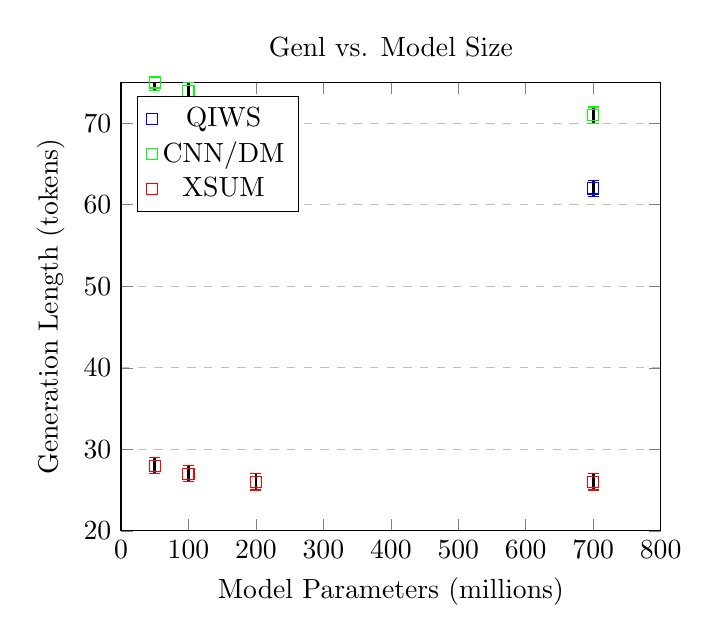
\begin{tikzpicture}
    \begin{axis}[
        title={Genl vs. Model Size},
        xlabel={Model Parameters (millions)},
        ylabel={Generation Length (tokens)},
        xmin=0, xmax=800,
        ymin=20, ymax=75,
        xtick={0, 100, 200, 300, 400, 500, 600, 700, 800},
        ytick={20, 30, 40, 50, 60, 70, 80},
        legend pos=north west,
        ymajorgrids=true,
        grid style=dashed,
    ]
    
    % QIWS data points
    \addplot[
        color=blue,
        mark=square,
        only marks,
        error bars/.cd,
        y dir=both,
        y explicit,
        error bar style={line width=1pt, draw=black},
    ]
    coordinates {
        (50, 62) +-(0, 1)
        (100, 62) +-(0, 1)
        (200, 62) +-(0, 1)
        (700, 62) +-(0, 1)
    };
    \addlegendentry{QIWS}
    
    % CNN/DM data points
    \addplot[
        color=green,
        mark=square,
        only marks,
        error bars/.cd,
        y dir=both,
        y explicit,
        error bar style={line width=1pt, draw=black},
    ]
    coordinates {
        (50, 75) +-(0, 1)
        (100, 74) +-(0, 1)
        (200, 72) +-(0, 1)
        (700, 71) +-(0, 1)
    };
    \addlegendentry{CNN/DM}
    
    % XSUM data points
    \addplot[
        color=red,
        mark=square,
        only marks,
        error bars/.cd,
        y dir=both,
        y explicit,
        error bar style={line width=1pt, draw=black},
    ]
    coordinates {
        (50, 28) +-(0, 1)
        (100, 27) +-(0, 1)
        (200, 26) +-(0, 1)
        (700, 26) +-(0, 1)
    };
    \addlegendentry{XSUM}
    
    \end{axis}
\end{tikzpicture}

\end{document}